\documentclass[thesis.tex]{subfiles}

\begin{document}
\chapter{Discussion}
\label{sec:discussion}
We will in this chapter discuss the results which were presented in the preceding chapters. \textcolor{red}{MORE}
\section{Is the approach correct?}
We start by discussing the results from Chapter \ref{sec:validation}. Every test case in the chapter comes with a set of formal statements regarding the provided visualization, which represents the underlying result. We are not interested in arguing whether these statements are true or not: We want to discuss if the statements provide a valid basis for confirming the correctness of the approach. \\
\par\noindent
In the introduction of the chapter we describe omitting trivial statements to avoid tedious lists of uninteresting properties. By classifying a distinct set of traits as trivial we implicitly classify another, disjoint set as non-trivial. We have not chosen statements from this set exhaustively: We have chosen a set of statements which we consider to be non-trivial, but still general enough to describe the properties of the most fundamental, underlying, mathematical version of the alignment problem. When we envision the approach being utilized for a specific biological problem we would assume the need for a more specific set of statements. These could stem from domain knowledge from the exact biological question being answered, such as "Every valid alignment should only contain vertices from a separable subset of the population represented in the graph". Or they could originate from a statistical analysis point of view, for instance "The fraction of input sequences traversing a path should impact the alignment score of every alignment against that path". We claim these statements are unambiguously extensions to the set of statements provided in this thesis, and thus they strictly represent further specifications of the problem being solved. Although they might be necessary adjustments to turn the approach into an applicable solution to real life problems, we argue the algorithm as presented here has an innate value in its universality, as a proof of concept: A basis easily modifiable for more specific scenarios. We conclude that the approach is correct for the problem is meant to solve, and although this problem is a simplified version it is situated at the core of more special applications.
\section{Is the approach efficient?}
We will move on to discuss the results found in Chapter \ref{sec:performance}. Specifically there are three complexity related characteristics with these results we find interesting: The efficiency of the approach under optimal conditions, the complexity in relation to introducing fuzzyness and the indexation. The three subsequent sections will summarize these characteristics, discuss the nature of their results and the effects this has on the viability of the approach. The results from the accuracy tests will be discussed separately in section \ref{sec:heuristical_applications} and also to a large degree form the fundament for possible future work discussed in Chapter \ref{sec:future_work}.
\subsection*{Optimal conditions}
We define the base case in the experiments done as the problem of aligning an unaltered read back to its origin. We test this by putting constraints on the parameters concerned with fuzzyness and vary the remaining variables, typically related to the complexity of the input data. The results can be seen in figures \ref{fig:runtime_G}, \ref{fig:runtime_s} and \ref{fig:runtime_b}. The first set of tests were concerned with determining the relationship between execution time and the number of vertices in the graph. As expected PO-MSA shows a clear linear relation over the entire sample. The fuzzy search is only dependant on the graph size to determine the depth of the suffix tree which is searched, and this logarithmical relationship looks almost constant in comparison. In the tests examining different sequence lengths we also see a much smaller growth in our approach then what can be seen in PO-MSA, although both appear to be linear. The reason for the different linear factors can be caused by the number of vertices which are traversed by the exhaustive search. Every such vertex has to do a number of operations correlated to the sequence length, reducing this number should impact the total number of operations necessary. The tests concerned with branching factor shows no distinct indications on which approach should be preferred.\\
\par\noindent
The results from these three tests leads us to conclude that the fuzzy search algorithm outperform PO-MSA by a large factor in what we have defined as the base cases: Aligning an unaltered read back to its origin. This in itself is not an extremely impressive result: It can be achieved through simpler solutions, for instance by using hashed k-mers of length $|r|$ from the graph as an index. What is interesting is that this is not the characteristic which was identified as the goal of the approach and then sought out in a vacuum: It emerges from a solution to a more general problem. This shows the approach is very tractable for the simplest use cases.
\subsection*{The exponential growth in relation to fuzzyness}
We increase the complexity of the test cases by introducing fuzzyness through the error margin parameter $\lambda$. The results can be seen in figure \ref{fig:runtime_lambda}, where a large exponential growth is displayed. This is in a way expected: Fuzzyness has the innate property of exponentially increasing the number of interesting possibilities. When we combine this with a dense search space of similar sequences the growth explodes. At some point it is better to exhaustively let PO-MSA test the possibilities we actually have instead of letting the fuzzy search generate and search for variants. The border between the two is represented where the two functions cross in the figure.\\
\par\noindent
The extreme growth and the early cross over point between the two algorithms in the figure indicate that our approach have limited applications when faced with large amounts of variation. In figure \ref{fig:runtime_lambda_parallell} there are results which can refute this conclusion to some degree. We can see that a simple parallellization seem to put a linear bound on the exponential growth. There still exists room for large optimizations through parallellizing the suffix tree search\footnote{These possibilities are further discussed in chapter \ref{sec:future_work}}; we included a simple version to display the powerful effect. However, the most important point seen in relation to graph size: Although the growth is bad, the starting point is decided by the ``base case'' of no fuzzyness, a behaviour we know will improve as the size of the input data increases. Figure \ref{fig:projected_lambda} shows the results from the larger data set projected onto the plot displaying the results from the smaller data set\footnote{The results seen in figures \ref{fig:runtime_lambda} and \ref{fig:runtime_lambda_parallell}}. The fact that these two factors do not seem to interact with each other results in an increase in tractability as the data sets grow: A very desirable trait when dealing with real genetic data. 

Another important argument can be made as the graph size increases in comparison to the read length. There will exist a larger number of pure combinations of paths of length $|r|$ in the graph, which decreases the probability of not finding anything relevant. This in turn leads to a decreased need for a high $\lambda$ value. These two pieces of information leave us arguing that the approach still present interesting opportunities when dealing with real data.
\begin{figure}
  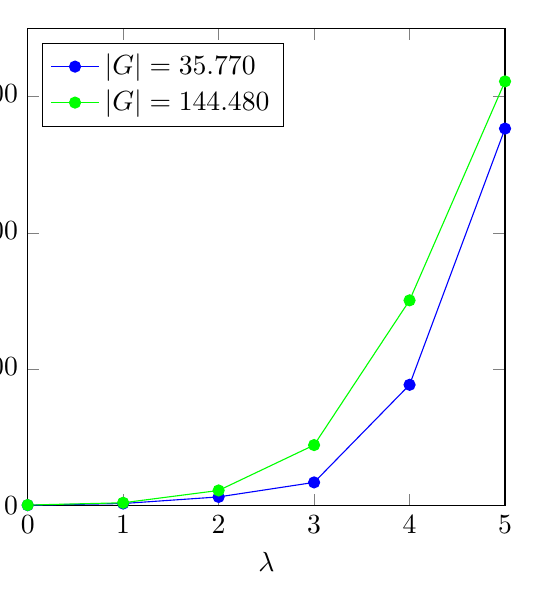
\begin{tikzpicture}[trim axis left, trim axis right]
    \begin{axis}[scale only axis,height=0.5\textwidth,width=0.5\textwidth,xmin=0,ymin=0,xmax=5,ymax=35000,scaled ticks=false, legend pos=north west, xlabel={$\lambda$}, ylabel={Milliseconds},xtick={0,1,2,3,4,5}, legend cell align=left, ylabel near ticks]
      \addplot[color=blue,mark=*] coordinates {
        (0, 29)
        (1, 152)
        (2, 636)
        (3, 1700)
        (4, 8856)
        (5, 27642)
      };
      \addplot[color=green,mark=*] coordinates {
        (0, 39)
        (1, 207)
        (2, 1109)
        (3, 4438)
        (4, 15048)
        (5, 31101)
      };
\addlegendentry{$|G|=35.770$}
\addlegendentry{$|G|=144.480$}
\end{axis}
\end{tikzpicture}
\caption{}
\label{fig:projected_lambda}
\end{figure}
\subsection*{Indexation}
The possibly most visually outstanding result presented in the previous chapter is the pure amount of time used by the indexation process, as seen in figures \ref{fig:index_constituents_explicit} and \ref{fig:comparison_align}. Most of this time is used by slow interactions with the file system, by reading and writing a large index. This thesis has not at all been concerned with the tractability of this process. Although the results seem severe there exists solutions both for better compression \cite{a_block_sorting_lossless_data_compression_algorithm}\cite{compression}, better serialization\textcolor{red}{[ref]} and smarter interactions with slower hardware\textcolor{red}{[ref]}. Ultimately one could argue that in a real life scenario the index should be kept in memory on a supercomputer\textcolor{red}{[ref]}\textcolor{red}{[ref]}. Importantly, we are not concluding that it is fair to completely remove the indexation factor when examining the results. We are rather stating this is a key component of the developed approach, but the work is left for others.
\section{A comparison between the sequence graphs tool and the "fuzzy context-based alignment" tool}
\label{sec:conceptual_comparison}
In the previous chapter we presented some results from a set of tests run as a comparison between the sg tool and our tool. We made some arguments as to why this comparison was hard to do, and what problems we were faced with. Because of these, we will in this section focus on the conceptual differences in the two algorithms and the impact the divergence between them have on the results, both in light of the alignments they produce and what differences in time complexity can be expected. We will start by describing the approaches step by step to have a more detailed picture when doing comparisons. Throughout this section we will refer to the approach developed by Novak et al. as sg and our approach as fuzzy search.\\
\par\noindent
Both algorithms start out by searching for contexts. Already here there is a separation through the requirement for uniqueness, but we see this as a clear design choice taken based on domain knowledge. When we also take into account the previously described triviality of changing between the two choices we see this as a difference which is not that interesting in this setting. When the contexts have been found, the algorithms start to diverge. The fuzzy search picks out the vertice in ``center'' of the context and stores it in a candidate set. We later search through the candidate sets with an exhaustive search algorithm. Sg locks the entire context on to the string and seeks to increase the locked portion by combining overlapping contexts. The overlapped contexts are further expanded by combining them with allowed gaps in between, and finally doing a bounded search to fill in the remaining gaps.\\
\par\noindent
We can go further in comparing the two by describing the sg algorithm in terms of the data structures used in describing our approach. Because of the uniqueness restriction, each candidate set would either contain a single vertex or be empty. Both singular contexts and the combination of these would be represented by consecutive candidate sets containing consecutive vertices. The second search done to combine non-overlapping contexts would be similar to the search we do, a bounded search seeking to find ``missing'' candidate vertices for a short consecutive number of candidate sets. The final search is required when we have consecutive empty candidate sets spanning a number of indexes larger than a given mismatch parameter. This search could for instance be implemented as a PO-MSA search starting in the vertex in the last non-empty candidate set preceding the gap and ending in the vertex in the first non-empty candidate set succeding the gap.\\
\par\noindent
When we have both algorithms on this level of detail the separation between them becomes apparent. Our approach is based on the assumption that \textit{if we localize all interesting areas, an optimal solution is bound to be in the combination of them}. The sg approach seems based on an assumption along the lines of \textit{if we find enough uniquely identifiable areas, we can combine these into a good solution}. We can see a clear cut distinction between a non-heuristical and an heuristical approach, which will have an effect on the quality of the results. There are two points which separate the algorithms in regards to runtime: Firstly, we search for a complete number of candidates, a number which grows exponentially related to the allowed fuzzyness. We also do an exhaustive search on all the possible recombinations, another exponential factor. The results from this separation should become apparent in both algorithms when faced with non-optimal cases, represented by searching for strings which do not have a good counterpart in the graph. Sg would see a decrease in quality of the results while we see a growth in runtime. Both can argue these are cases they are not meant specifically to handle. \textcolor{red}{Transition}.
\section{Heuristical applications}
\label{sec:heuristical_applications}
We first presented the possibilities for finding heuristical alignment which showed themselves through our algorithm in section \ref{sec:heuristical_conceptual}. We described our exploration of these possibilites through the \texttt{-{}-heuristical=true} parameter in the GraphGenome tool in section \ref{sec:implementation_heuristic}. For reasons previously discussed we moved away from the realm of heuristics through the chapters concerned with testing, except for a brief comparison with the regular algorithm related to accuracy. We will now return to once again considering the viability of this modified approach. The motivation behind this discussion becomes obvious when examining the results: The largest drawback with the approach is the explosive growth in complexity in relation to introduced fuzzyness. In figure \ref{fig:correctness} we can see that when the algorithm is run with the \texttt{-{}-heuristical=true} parameter it does not show the same directly linear correlation between the amount of noise and $\lambda$. If we can avoid a high error margin, we can avoid the problems brought on by the exponential growth. Showing the validity of the heuristical approach is thus equivalent with significantly increasing the tractability of the approach.\\
\par\noindent
Introducing heuristics is usually done to improve computational tractability, often at the cost of ambiguity: You can no longer assure the found result is correct. The approach we propose in this thesis will only run heuristically when no optimal alignment is found within the constraints of the regular algorithm. This means that for every input triplet ${G, s, T}$, where there actually exists an optimal alignment A with a score higher than $T$, the algorithm will run non-heuristically and thus guarantee optimality. We can even show this holds for results which has a score of $T-1$: If there existed an alignment with score $T$ we would have found it. There can be no alignment scoring better than $T-1$ and worse than $T$\footnote{Assuming integer scores}. Thus what we have found must be optimal. Whenever we move beyond $T-1$ we can no longer say anything about the optimality of the achieved result, but we can to some degree guarantee it is a product of smaller optimal solutions. More verbally this can be formulated as \textit{If there exists a good enough alignment the algorithm will find it, if not the algorithm will make an educated guess}. There is even an option of defining what is ``good enough'' through the input variable $\lambda$. We claim this is a level of precision attractive to any heuristical algorithm.
\section{Conclusion}
The aim of this thesis was to present the approach we developed, and through testing its validity and efficiency determine whether it represents a feasible solution to the problem of aligning text strings against graphs. We have shown that the implementation provides expected results and argued for the validity of these results as a solution to the most general form of the problem. The performance results were more ambiguous, revealing that the algorithm has both strengths and weaknesses. We have discussed both of these in this chapter, while also proposing possible solutions to some of the arising problems. The fact that there still are shortcomings leads us to conclude that our approach can not serve as an optimal solution to the alignment problem. However, because of the feasibility of the heuristically modified algorithm, we do argue it is an important step along the way to this goal. We will briefly present our thoughts on where this path could lead in the subsequent chapter.
\end{document}
